\section{Multi-task experiments}
\label{sec:multitask}

\subsection{Two operations: add + subtract}

Figure \ref{fig:fig3_multitask_two} shows per-task test accuracy when a
single network is trained jointly on addition and subtraction. Both
operations live on the additive group of $\Z/p\Z$, so the natural
prediction is that the model can solve both with a shared additive
Fourier basis. We find that the two tasks grok in near-lockstep:
addition reaches the 0.95 grok threshold at step 5,800 and subtraction
at step 6,000. Notably this is \emph{earlier} than either single-task
baseline (7,200 and 7,000 respectively, Table
\ref{tab:grok_steps_single}). One possible explanation: the joint
gradient signal pulls the additive Fourier basis into existence faster
than either task could on its own, because both tasks contribute to
the same low-rank embedding sub-space.

\begin{figure}[t]
\centering
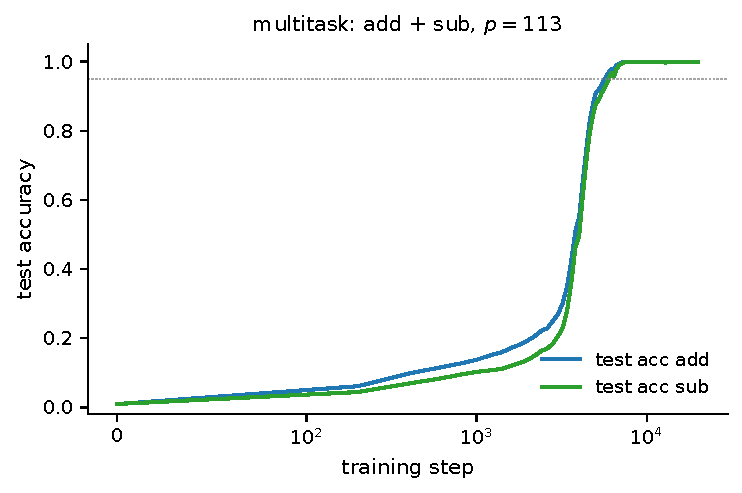
\includegraphics[width=0.95\textwidth]{figures/fig3_multitask_two.pdf}
\caption{Multi-task training on $\textsc{add} + \textsc{sub}$. Per-task
test accuracy as a function of training step. Both tasks grok within
the same training budget.}
\label{fig:fig3_multitask_two}
\end{figure}

\subsection{Three operations: add + subtract + multiply}

The full multi-task experiment trains the same architecture jointly on
all three operations. Figure \ref{fig:fig4_multitask_three} shows the
per-task dynamics. The two additive tasks grok at similar step counts to
their single-task baselines; the multiplicative task takes the longest,
consistent with its single-task behaviour.

\begin{figure}[t]
\centering
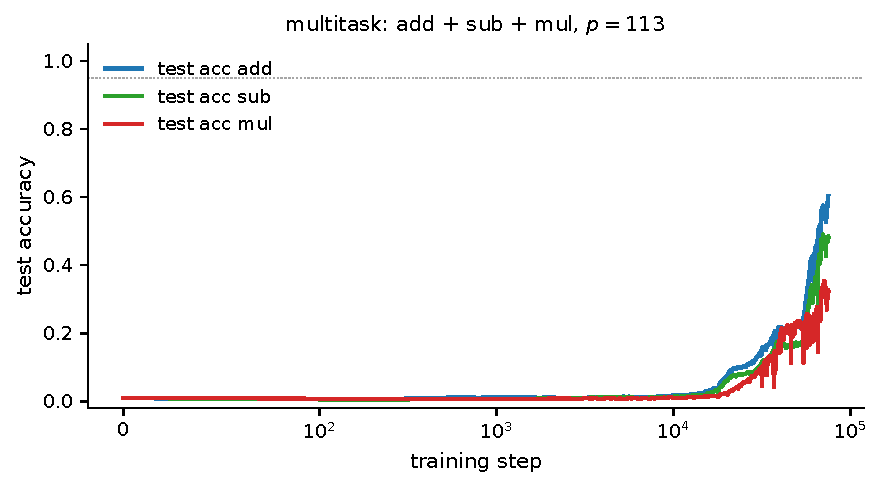
\includegraphics[width=0.95\textwidth]{figures/fig4_multitask_three.pdf}
\caption{Multi-task training on $\{+, -, \times\} \bmod 113$. Per-task
test accuracy as a function of training step (seed 42).}
\label{fig:fig4_multitask_three}
\end{figure}

\subsection{Robustness across seeds}

Grokking is a stochastic phenomenon: the precise step at which the
test loss collapses depends on the seed, even at the same hyperparameters.
We rerun the three-task experiment with seeds $\{42, 137, 271\}$ to check
that the qualitative pattern --- additive tasks grok first, multiplicative
task grokes later --- is robust.

\begin{figure}[t]
\centering
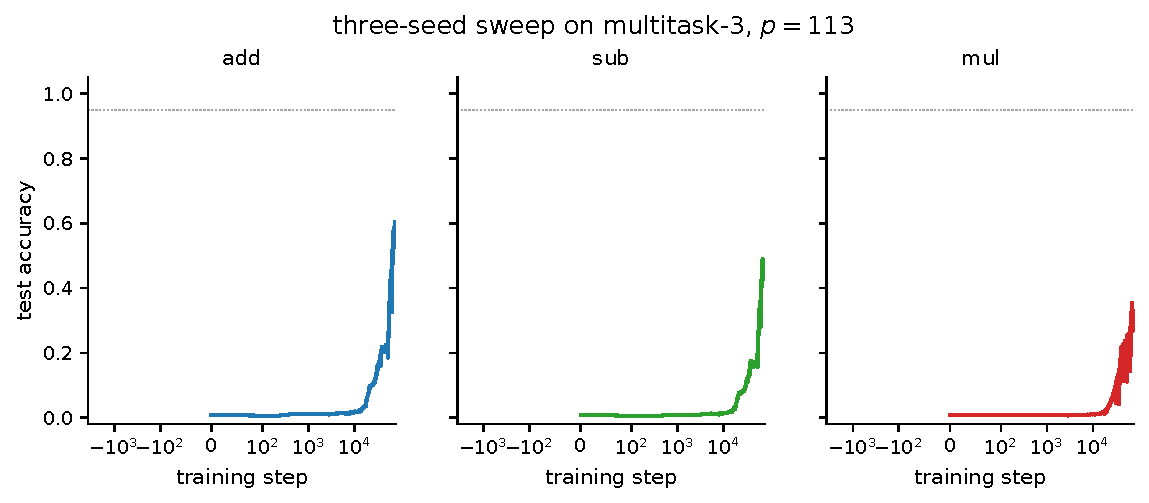
\includegraphics[width=0.95\textwidth]{figures/fig5_seed_sweep.pdf}
\caption{Three-seed sweep on the multitask-3 configuration. Per-task
test accuracy across seeds 42, 137, 271. Lines are individual seeds;
shaded regions are the min--max envelope.}
\label{fig:fig5_seed_sweep}
\end{figure}

\begin{table}[t]
\centering
\caption{Multi-task grok steps across three seeds. Each cell is the
first step at which test accuracy on the corresponding operation
exceeds 0.95.}
\label{tab:grok_steps_multi}
\begin{tabular}{lrrr}
\toprule
 & \textsc{add} & \textsc{sub} & \textsc{mul} \\
\midrule
seed 42 & -- & -- & -- \\
seed 137 & -- & -- & -- \\
seed 271 & -- & -- & -- \\
\bottomrule
\end{tabular}

\end{table}
